\documentclass[letterpaper,10pt,conference]{ieeeconf}
\IEEEoverridecommandlockouts
\overrideIEEEmargins
\usepackage{fontspec}
\setmainfont{Times New Roman}\setsansfont{Arial}\setmonofont{Menlo}
\usepackage{amsmath,amssymb,graphicx,booktabs,cite,url}
\graphicspath{{figures/}}
\newcommand{\vct}[1]{\vec{#1}}
\newcommand{\BudgetSpeed}{$0.283\,\mathrm{m/s}$}
\newcommand{\WalkSpeed}{$0.126\,\mathrm{m/s}$}
\newcommand{\AbstractRateResult}{The maximum sector-command rate decreases from 1517 to 536 degree/s relative to the original allocator, retaining 99.95\% of its mean forward speed.}

\title{\LARGE\bf Rewind-Budgeted Contact-Travel Allocation\\for an Articulated Arc-Leg Hexapod}
\author{\mbox{}}
\begin{document}
\maketitle\thispagestyle{empty}\pagestyle{empty}
\begin{abstract}
An articulated leg with a finite circular arc can transport its body through both joint articulation and distal rolling. The available rolling stroke, however, is limited by how far the arc can be rewound during a subsequent swing. We present a contact-travel allocator that couples this rewind budget to rolling and stepping roles on an eighteen-actuator hexapod. A quintic swing profile yields an explicit sector-excursion bound, while a discrete slew guard covers interrupted swing windows. The articulated trajectory supplies the travel remaining after the bounded rolling increment. We evaluate seven controller restrictions in MuJoCo and extend the comparison to reverse, lateral, turning, model-parameter stress, collision representation, and timestep conditions, totaling 268 prescribed trials. At a forward command of 0.45 m/s, the proposed controller achieves \BudgetSpeed{} compared with \WalkSpeed{} when rolling is disabled. \AbstractRateResult{} A 24-piece convex decomposition preserves the tire's inner cavity and supports the primary comparisons. The study identifies the transport and feasibility trade-offs of finite-sector allocation; archival prototype footage provides mechanical context, while quantitative validation of the proposed controller on hardware remains future work.
\end{abstract}

\section{Introduction}
Rolling contacts and articulated legs provide complementary ways to move a robot. Rolling can transport the body without consuming a large articulated stride, while upstream joints can place a contact beyond its current support region. When a finite arc replaces a complete wheel, these functions share one distal joint. This actuator reuse is attractive, but it also couples stance transport to the motion required to restore the arc for its next contact.

A finite arc has two distinct angular constraints. Its remaining tread limits how far it can rotate while supporting the body. Its swing duration and allowed angular rate limit how far it can be rewound before touchdown. A controller can respect the first constraint and still violate the second. In addition, simply adding rolling to a full walking trajectory can assign the same contact travel to both mechanisms. The resulting conflict depends on steering alignment and the articulated workspace; it cannot be resolved by increasing distal rotation alone.

We address these constraints through a common body-relative contact-travel budget. Geometry determines which legs can roll in a useful direction. A bounded sector increment supplies part of the required travel, and articulation supplies the residual. The sector excursion is additionally limited by the distance that a quintic swing can rewind. Roles and steering are adopted at lift-off, allowing the corner legs to roll while the middle pair steps under a forward command. Figure~\ref{fig:platform} shows the physical embodiment and the corresponding model.

The contributions are threefold. First, we formulate a rewind-aware allocation rule with an explicit sector-excursion bound and a discrete sector-rate invariant. Second, we implement the rule in a common position-control path and isolate travel subtraction, reindexing, scheduling, and the rewind guard through seven controller restrictions. Third, we evaluate the resulting trade-offs on a frozen simulation revision with a concavity-preserving contact approximation, paired initial phases, additional command directions, and numerical sensitivity checks. The contribution concerns a finite-sector control mechanism on one articulated morphology. It does not depend on claiming that curved legs, actuator reuse, or hybrid locomotion are new.

\begin{figure}[t]
\centering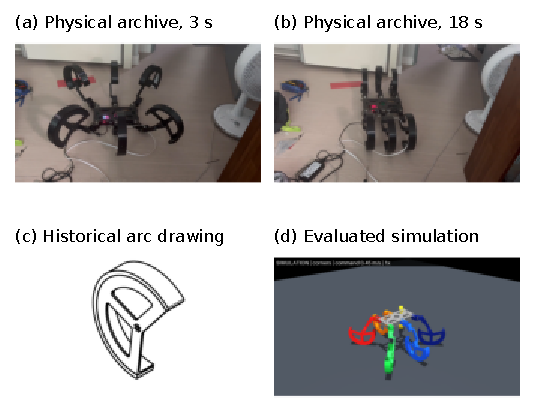
\includegraphics[width=\columnwidth]{platform.pdf}
\caption{Arc-leg embodiment and model. (a,b) Archival floor-motion frames at source times 3 and 18 s. (c) Historical arc fabrication drawing. (d) Nominal simulation pose. The physical clips use an undocumented historical controller and include external cables; they are not hardware trials of the proposed allocator.}
\label{fig:platform}
\end{figure}

\section{Related Work}
RHex established the mobility of a hexapod with continuously rotating compliant curved legs~\cite{saranli2001rhex}. Q-Whex further develops quasi-wheeled hexapod motion~\cite{zhang2023qwhex}. Energy-oriented design guidelines and kinematic studies also connect C-leg geometry to locomotion performance~\cite{vina2021cleg,burzynski2024kinematics}. These systems motivate efficient use of curved contacts, while the present problem concerns an arc mounted after two additional articulated joints and restricted to a bounded position range.

Transformable leg-wheel robots provide the closest morphological context. Quattroped shares actuation across wheel and leg configurations~\cite{chen2014quattroped}, and TurboQuad addresses smooth behavioral transitions~\cite{chen2017turboquad}. R-Taichi studies rolling and swing strategies on a transformable two-degree-of-freedom limb, including physical experiments~\cite{xue2025rolling}. Chang and Lin describe stride-level hybrid locomotion with aerial repositioning and energy-oriented optimization~\cite{chang2026stride}. Accordingly, combining rolling and swing within a stride is established. Our narrower question is how to bound the rotation of a fixed finite sector by its available rewind interval and allocate the remaining contact travel to articulation.

Articulated wheel-leg platforms also coordinate contact placement and rolling, including ASTERISK H~\cite{yoshioka2008asterisk}, whole-body wheeled-quadruped control~\cite{bjelonic2019keep}, and online gait-sequence generation with model predictive control~\cite{bjelonic2021wholebody}. These methods address broader force and motion planning problems. Our allocator uses geometric roles and position targets without online force optimization or learned policies. The experiments therefore test its internal mechanisms under a common embodiment and motor setup, rather than claim superiority over whole-body controllers on different robots.

Repeatable testing matters when small control changes alter contact sequences. Weng et al.~\cite{weng2024testing} demonstrate the importance of controlled conditions in legged-robot evaluation. We use fixed paired phases and explicit parameter stress conditions, report failures as well as transport, and distinguish these deterministic comparisons from hardware reliability estimates.

\section{Platform and Contact Representation}
\subsection{Embodiment and Actuation}
The model is a hexapod with three revolute joints per leg and eighteen actuators. The upper joint steers the limb about a vertical axis; two downstream joints articulate the leg, and the distal joint rotates the arc. The model mass is 4.161 kg. The tire envelope has an outer radius of 122.5 mm, an inner radius of 112.5 mm, and a width of 44 mm. Dimensions in the historical drawing provide manufacturing context but do not calibrate the compliance of the simulated tire.

Every condition uses the same floating base, inertias, controller gains, voltage limits, and nominal pose. The actuator path computes a proportional-derivative torque request and a bounded voltage command,
\begin{align}
 \tau_j^c&=k_{p,j}(q_j^\star-q_j)+k_{d,j}(\dot q_j^\star-\dot q_j),\\
 V_j&=\operatorname{sat}_{[-12,12]}[(R_j/K_j)\tau_j^c+K_j\dot q_j].
\end{align}
Reflected rotor inertia is included. The common gait setup disables the additional target-profile velocity and acceleration limiter and doubles the middle-joint proportional gain, with damping scaled by $\sqrt{2}$. Voltage and torque limits remain active. Thus the rate studied below is an explicit sector-command constraint, not a measured actuator capability or a guarantee on the total articulated joint rate.

\subsection{Contact Geometry and Rolling Direction}
Let $\vct{a}_i$ be the distal axis, $\vct{o}_i$ a point on it, and $\vct{p}_{c,i}$ the geometric support centroid. The planar material velocity induced by unit distal rotation is
\begin{equation}
 \vct{t}_i=\vct{a}_i\times(\vct{p}_{c,i}-\vct{o}_i),\qquad
 r_i=\|\vct{t}_{i,xy}\|.\label{eq:tangent}
\end{equation}
The geometric lowest point can remain almost stationary while successive material points move through contact. Its finite difference therefore does not identify the rolling direction. We instead use the axis-based tangent in~\eqref{eq:tangent}.

A geometric scan of the nominal standard pose gives usable sector offsets of $[-100^\circ,100^\circ]$ after margins. Across six legs and 21 offsets per leg, the lowest-patch centroid changes by at most 2.828 mm horizontally and 0.053 mm vertically. The centroid includes mesh vertices within 0.1 mm of the minimum height. This geometric check motivates adding a sector offset to an articulated IK solution, subject to the limits of a rigid contact approximation.

\subsection{Preserving the Inner Cavity}
Ordinary MuJoCo mesh collision uses a convex representation~\cite{mujococollision}. One mesh per tire therefore fills its annular interior, despite rendering an open arc. We replace the active tire contact by a union of convex parts generated with CoACD~\cite{wei2022coacd}. The original mesh remains visual geometry, and explicit body mass and inertia are unchanged. CoACD 1.0.14 uses a 2 mm real-metric concavity threshold and a fixed seed, yielding 24 parts per tire.

An independent probe places a sphere of radius 1 mm at the axle center. The single-hull representation reports contact at approximately $-23$ mm signed distance; the decomposition reports no contact. Over 720 planar directions, the change in the support function is below 0.004 mm. The summed convex-part volume exceeds the original mesh volume by 2.76\%, so the representation remains approximate. These checks verify a preserved cavity and essentially unchanged outer-plane support, rather than exact reproduction of all concave collisions or soft-tire deformation.

\begin{figure}[t]
\centering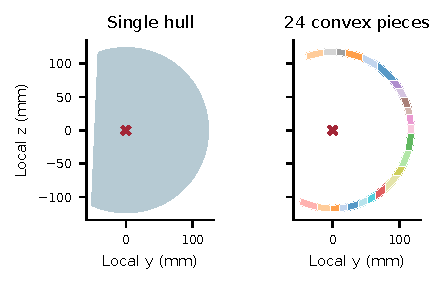
\includegraphics[width=\columnwidth]{collision.pdf}
\caption{Tire collision cross-section from actual mesh data. The single hull (left) fills the cavity. The 24-piece approximation (right) leaves the axle-center probe free while preserving the outer support envelope. Colors distinguish convex pieces; both models retain the same inertial properties.}
\label{fig:collision}
\end{figure}

\section{Rewind-Budgeted Travel Allocation}
\subsection{Steering and Contact Roles}
For a filtered body command $\vct{c}=[v_x,v_y,\omega_z]^\top$, the required contact travel in the body frame is
\begin{equation}
 \vct{u}_i=-[v_x-\omega_z y_i,\ v_y+\omega_z x_i]^\top,\label{eq:travel}
\end{equation}
where $[x_i,y_i]^\top$ is the nominal contact relative to the footprint centroid. We evaluate both distal rotation signs, clip steering to $\pm35^\circ$, and choose the direction $\hat{\vct{d}}_i$ with greatest alignment to $\vct{u}_i$. A leg qualifies for rolling when the alignment is at least 0.70; fewer than two qualifying legs causes an all-stepping assignment. Under forward motion, this geometry selects legs $\{1,2,5,6\}$ to roll while $\{3,4\}$ step (Fig.~\ref{fig:concept}).

\begin{figure}[t]
\centering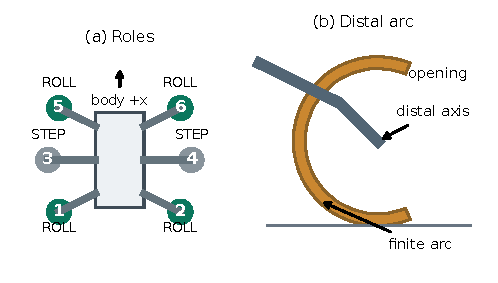
\includegraphics[width=\columnwidth]{concept.pdf}
\caption{Role allocation and finite distal arc, shown schematically. The upper joint changes both rolling heading and foot location. Roles and steering are therefore latched at lift-off. IDs follow the model convention.}
\label{fig:concept}
\end{figure}

\subsection{Rewind Distance and Sector-Rate Bound}
The alternating tripods $\{1,4,5\}$ and $\{2,3,6\}$ have phase offsets of one half-cycle. Frequency $f$ and duty factor $D$ give a swing duration $T_s=(1-D)/f$. A sector rewind from $\theta_{\rm lo}$ to a fixed home $h_i$ uses
\begin{equation}
 \theta(s)=\theta_{\rm lo}+S(s)(h_i-\theta_{\rm lo}),\quad
 S(s)=10s^3-15s^4+6s^5,
\end{equation}
with $s\in[0,1]$. Since $S'(s)=30s^2(1-s)^2$ has maximum $15/8$, a complete swing satisfies $|\dot\theta|\le\Omega$ if
\begin{equation}
 |\theta_{\rm lo}-h_i|\le B,\qquad B=\frac{8}{15}\Omega T_s.\label{eq:budget}
\end{equation}
For $f=2$ Hz, $D=0.60$, and $\Omega=540^\circ$/s, the rewind budget is $B=57.6^\circ$. This is smaller than the geometrically available sector excursion. We use $h_i=0$, which lies in every evaluated sector interval.

During stance, the next sector target is projected into the intersection of its geometric interval and rewind budget:
\begin{equation}
 \theta_{i,k+1}=\Pi_{[\ell_i,u_i]\cap[h_i-B,h_i+B]}
     (\theta_{i,k}+\Delta t\,\omega_{i,k}).\label{eq:project}
\end{equation}
The proposed rate $\omega_{i,k}$ is itself bounded by $\Omega$. For a state already in this interval, projection cannot increase the step magnitude beyond $\Omega\Delta t$. Thus stance respects both the excursion and discrete rate bounds. In swing, we apply an additional projection onto $[\theta_{i,k}-\Omega\Delta t,\theta_{i,k}+\Omega\Delta t]$. This slew guard preserves the discrete sector-rate invariant even when a swing is interrupted or resumed. The complete-swing premise in~\eqref{eq:budget} is required for reaching home within $T_s$; the slew guard alone does not guarantee that endpoint under interruptions.

A rolling leg decides whether to reindex at swing-window entry, based on spent reserve, loss of alignment, or predicted exhaustion before its next opportunity. For a locally constant sector rate, skipping the current window predicts $\theta_i^+=\theta_i+\omega_i/f$. If this value lies outside the intersection in~\eqref{eq:project}, the leg reindexes now. This one-cycle lookahead is a scheduling heuristic under changing commands, while the excursion and slew bounds remain explicit. This avoids starting a quintic trajectory midway through its allotted window. Roles are updated at actual lift-off. A stepping leg uses every swing window; rolling legs can skip unneeded swings. The schedule leaves at least three legs commanded in stance, while the number of loaded contacts is measured separately.

\subsection{Allocation After Saturation}
Before angular projection, the requested rolling speed is the projection of contact travel onto the steered rolling direction, scaled by an authority $\beta_i$. Authority fades over the last $12^\circ$ of the geometric interval. After~\eqref{eq:project}, articulation receives the residual based on the increment that will actually be commanded:
\begin{equation}
 \vct{u}^{\rm art}_i=\vct{u}_i-
 s_i r_i\frac{\theta_{i,k+1}-\theta_{i,k}}{\Delta t}\hat{\vct{d}}_i,\label{eq:residual}
\end{equation}
where $s_i$ maps the selected motor sign to rolling direction. This subtraction prevents the walking trajectory from requesting travel already assigned to rotation. Using the pre-saturation request would leave an unaccounted residual once the rewind budget is exhausted.

The residual is integrated into a stance offset, bounded by a 90/70 mm longitudinal/lateral elliptical workspace. Numerical IK generates articulated targets with a $40^\circ$ distal-branch guard and stride backoff when needed. The sector offset is added to the distal target, and final targets are clipped to $[0^\circ,360^\circ]$. The allocation equality describes commanded kinematics before workspace and final motor clipping; tracking lag and slip need not satisfy it. In particular, the summed distal target contains both IK and sector motion. The sector-rate invariant is not a bound on that sum.

\begin{figure*}[t]
\centering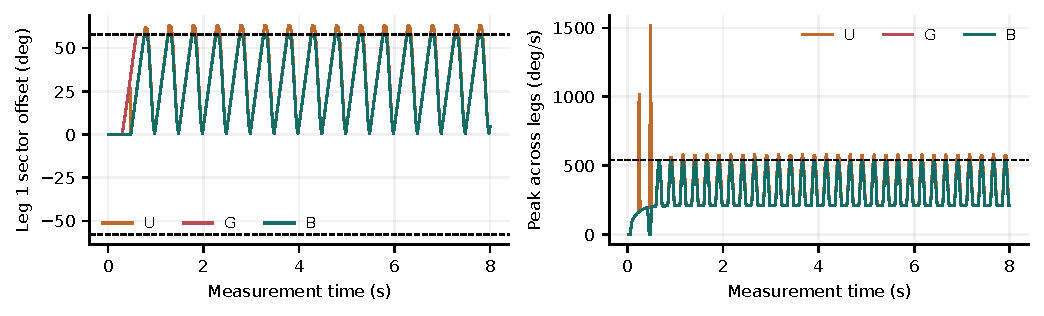
\includegraphics[width=.97\textwidth]{rate_budget.pdf}
\caption{Sector allocation in phase-zero, high-command trials. Left: leg-1 sector trajectories for U, B, and G; the G trace ends when its trial terminates. Right: maximum absolute sector rate across the six legs, with the prescribed 540 degree/s limit. These traces show the sector component of the command, before addition to the articulated distal target.}
\label{fig:rate}
\end{figure*}

\section{Experimental Method}
\subsection{Common Protocol and Restrictions}
We use MuJoCo 3.10.0~\cite{todorov2012mujoco}, a 2 ms physics step, and a 20 ms command update. Each fresh model is initialized, placed at the common nominal pose, and settled for 1 s before an 8 s measurement. The 0.15 s command filter and initial role-adoption transient are included. The maximum step height is 25 mm. There is no parameter retuning across conditions.

The main matrix compares the seven conditions in Table~\ref{tab:conditions} at forward commands of 0.18 and 0.45 m/s and initial phases $k/8$, $k=0,\ldots,7$, giving 112 trials. The primary geometry is the decomposed arc. U is the pre-guard travel allocator, while B adds the budget, fixed home, swing-entry decision, next-window lookahead, and slew guard together. Their comparison tests this complete rewind treatment, not an isolated projection operator. G removes the lookahead and tests whether a bounded excursion alone suffices for a reachable residual trajectory. The other restrictions retain B's settings.

\begin{table}[t]
\caption{Controller restrictions in the main comparison}
\label{tab:conditions}\centering\small
\begin{tabular}{cp{6.7cm}}\toprule
Code & Definition\\\midrule
U & Original allocation; geometric arc limits, original swing timing.\\
B & Proposed rewind-budgeted allocation.\\
G & B without the next-window budget lookahead.\\
N & B with all rolling roles disabled.\\
S & B with full articulated travel superposed on rolling; no subtraction.\\
D & B with rolling-leg reindexing disabled after role adoption.\\
P & B with periodic rolling-leg swings at every window.\\\bottomrule
\end{tabular}
\end{table}

An additional 84 trials compare B/N/S over seven commands: forward 0.30 m/s, reverse $-0.18$ m/s, lateral $\pm0.12$ m/s, yaw $\pm0.45$ rad/s, and a curve at 0.18 m/s with 0.35 rad/s yaw. Each uses four phases. Three separate stress settings---mass multiplied by 1.2, friction by 0.5, or actuator strength by 0.8---yield 36 high-command trials of B/N/S over four phases. These factors are declared numerical stress cases, not identified hardware uncertainty distributions.

We further repeat B/N/S on the single-hull geometry at both main commands and four phases (24 trials). Timestep checks use 1 and 4 ms at the high command and phases 0 and 0.5 (12 trials), paired with the existing 2 ms records. The complete design therefore contains 268 trials. The commands are constant within each trial; they do not establish closed-loop command-transition performance.

The source revision, dependencies, model and decomposition hashes, condition matrix, and output rules are fixed before the complete run. Raw failures are retained. A target rejected by the public sender because IK did not converge terminates its trial, as do nonfinite state and a body tilt exceeding $60^\circ$. Completion is reported independently of tracking accuracy. A development run exposed premature budget exhaustion without lookahead; this motivated B and the explicit G restriction. The reported matrix was then frozen and run in full. It is a confirmation of the revised mechanism, not an independently held-out benchmark. Earlier development results are not pooled with these summaries.

\subsection{Metrics}
Primary forward transport is the net displacement projected onto the initial chassis axis, divided by the measured duration. A world-frame velocity integral at the same root origin provides an independent cross-check in 20 separate validation replays. Translational and yaw-rate RMSE compare instantaneous body-frame motion with the original command, including startup transients. Failed trials have shorter durations and are reported as failures; their truncated speeds are not substituted for full-window averages.

We measure sector-command peak rate, peak excursion, and the number of command frames exceeding the 540 degree/s sector limit. We separately record the rate of the summed distal motor target. Loaded-leg count uses distinct tire bodies with normal contact force above 1 N, so subdividing a tire cannot create additional counted legs.

Absolute mechanical work is $W_{\rm abs}=\int\sum_{j=1}^{18}|\tau_j\dot q_j|dt$. Its transport normalization is $W_{\rm abs}/(mg\|\Delta\vct{p}_{xy}\|)$, using net planar displacement. This quantity is not battery energy. Slip integrates mean tangential velocity over loaded tire--ground contact points; it is neither load weighted nor independent of collision-point multiplicity. We consequently compare slip primarily within one geometry.

Phases are a deterministic grid rather than independent random samples. We report means, full observed ranges, and phase-paired differences without population confidence intervals. Positive transport or survival of the tilt threshold is insufficient evidence of reliable operation.

\section{Results}
\subsection{Rewind Feasibility and Forward Transport}
Table~\ref{tab:main} separates completion from full-window transport. B, U, N, and P complete all 16 main trials. At the high command, B reaches 0.283 m/s against N's 0.126 m/s, a factor of 2.25. The phase-paired B-minus-N gain averages 0.157 m/s and spans [0.151, 0.162] m/s. B retains 99.95\% of U's mean speed while reducing the maximum sector rate from 1516.8 to 536.4 degree/s. U exceeds the prescribed rate in every high-command trial; B has no violating frames in the main matrix.

\begin{table*}[t]\centering\small
\caption{Main matrix: completion and full-window speed, mean [minimum, maximum]}
\label{tab:main}
\begin{tabular}{cccccc}\toprule
 & \multicolumn{2}{c}{0.18 m/s command} & \multicolumn{2}{c}{0.45 m/s command} & High-command sector\\
Code & Complete & Speed (m/s) & Complete & Speed (m/s) & peak rate (degree/s)\\\midrule
U & 8/8 & 0.114 [0.113, 0.116] & 8/8 & 0.283 [0.278, 0.288] & 1516.8\\
B & 8/8 & 0.114 [0.113, 0.116] & 8/8 & 0.283 [0.280, 0.286] & 536.4\\
G & 8/8 & 0.114 [0.113, 0.116] & 0/8 & -- & 535.7\\
N & 8/8 & 0.094 [0.092, 0.095] & 8/8 & 0.126 [0.122, 0.129] & 0.0\\
S & 0/8 & -- & 0/8 & -- & 179.3\\
D & 0/8 & -- & 0/8 & -- & 203.0\\
P & 8/8 & 0.113 [0.111, 0.114] & 8/8 & 0.284 [0.281, 0.285] & 536.4\\
\bottomrule\end{tabular}
\par\vspace{5pt}\noindent\parbox{.96\textwidth}{\footnotesize Peaks for failed conditions cover only the interval before termination. A dash indicates that no trial completed the full 8 s; truncated speeds are not averaged into successful performance.}
\end{table*}

The distance-only restriction G completes the low-command trials but rejects an IK target in all eight high-command trials. Bounding sector excursion without anticipating the next swing can exhaust the rolling budget while the leg remains in stance; the resulting articulated residual becomes unreachable. Adding the lookahead in B restores completion for these trials. The full-superposition restriction S and disabled-reindexing restriction D reject targets in all main trials. These outcomes concern this posture, workspace, and command range; they do not imply that all superposed or nonreindexing controllers must fail.

Periodic scheduling P also completes all main trials and has essentially the same high-command speed as B. At the low command, B has only a small mean advantage. Thus these trials support the need for timely reindexing but do not establish adaptive scheduling as superior to periodic scheduling. The stronger contrast is rate feasibility against U, and reachable residual motion against G and S.

\begin{figure*}[t]\centering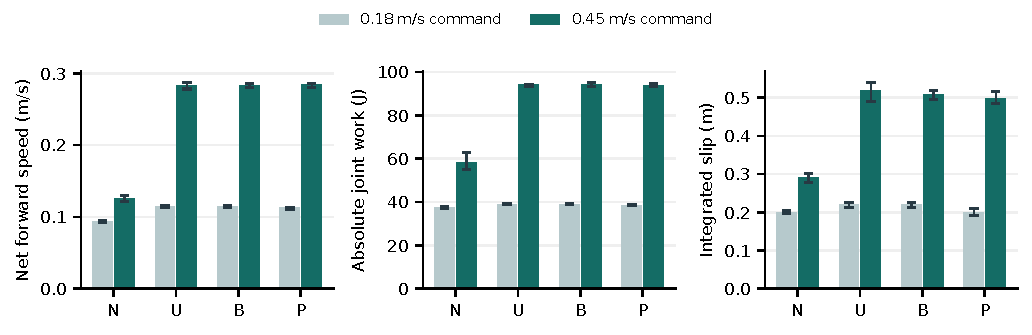
\includegraphics[width=.97\textwidth]{results.pdf}
\caption{Four conditions that complete every main trial. Bars are eight-phase means; whiskers are full phase ranges. G, S, and D are reported with their failures in Table~\ref{tab:main}. Faster transport is accompanied by changes in joint work and slip, so speed alone is not an efficiency result.}
\label{fig:results}\end{figure*}
\subsection{Work, Tracking, and Loaded Support}
At the high command, B uses 94.2 J of absolute joint work against N's 58.1 J. Integrated slip is 0.509 versus 0.290 m. Their respective translational RMSE values are 0.196 and 0.331 m/s. B therefore improves net transport without demonstrating uniformly lower work or slip. Its main trials include a minimum loaded-leg count of 1, and up to 11.65\% of physics samples have fewer than three. This illustrates why a three-leg stance schedule is not a three-contact load guarantee. The summed distal target reaches 1594.6 degree/s across the B trials, exceeding the sector-component bound; applying the method to a physical actuator requires a joint-level trajectory constraint.

\subsection{Commands Beyond Forward Motion}
Table~\ref{tab:domain} reports all seven additional commands. Translational and yaw errors are separate because a controller can remain upright while tracking poorly. Each comparison uses the same four initial phases. The results describe constant-command operating points, including cases where both B and N fall back to stepping.
\begin{table*}[t]\centering\small
\caption{Additional commands: completion and tracking error over completed trials}
\label{tab:domain}\begin{tabular}{lccccc}\toprule
Command $(v_x,v_y,\omega_z)$ & Complete B/N/S & B $e_v$ & N $e_v$ & B $e_\omega$ & N $e_\omega$\\\midrule
(0.3, 0, 0) & 4/4/0 & 0.124 & 0.177 & 0.084 & 0.086\\
(-0.18, 0, 0) & 4/4/0 & 0.078 & 0.097 & 0.058 & 0.036\\
(0, 0.12, 0) & 4/4/4 & 0.041 & 0.057 & 0.004 & 0.002\\
(0, -0.12, 0) & 4/4/4 & 0.042 & 0.057 & 0.005 & 0.002\\
(0, 0, 0.45) & 4/4/4 & 0.043 & 0.043 & 0.275 & 0.275\\
(0, 0, -0.45) & 4/4/4 & 0.042 & 0.042 & 0.274 & 0.274\\
(0.18, 0, 0.35) & 4/4/1 & 0.102 & 0.112 & 0.186 & 0.212\\
\bottomrule\end{tabular}
\par\vspace{5pt}\noindent\parbox{.96\textwidth}{\footnotesize Each completion count is out of four. $e_v$ is translational RMSE (m/s); $e_\omega$ is yaw-rate RMSE (rad/s). Units of the command are m/s, m/s, and rad/s. Failed-trial errors are not mixed with full-window errors.}
\end{table*}

\subsection{Parameter, Geometry, and Timestep Checks}
With 1.2-fold mass, B completes 4/4 trials and N completes 4/4. Their mean speeds are 0.270 and 0.118 m/s. With half nominal friction, B completes 4/4 trials and N completes 4/4. Their mean speeds are 0.316 and 0.134 m/s. With 0.8-fold actuator strength, B completes 4/4 trials and N completes 4/4. Their mean speeds are 0.293 and 0.130 m/s. These isolated stress cases are not a population robustness estimate.

For paired completed B/N trials, changing from decomposed contacts to the single hull changes net speed by at most 0.0122 m/s. The 1/2/4 ms comparison changes speed by at most 0.0008 m/s relative to 2 ms. These are local sensitivity results, not a proof of solver convergence or concave-edge accuracy. Contact-point slip is not compared across the two representations because decomposition changes the contact manifold.

Across the prescribed matrix, 193/268 trials complete; all incomplete trials terminate because an IK target is rejected. B completes 68/68 trials with 0 sector-rate violation frames. A separate 20-trial check integrates the velocity at the same root origin used for displacement. Its maximum speed discrepancy is 0.00009 m/s. Velocity at the body center of mass is retained as a diagnostic at a different point and is not substituted for velocity at the root origin. The three visual replays in Fig.~\ref{fig:replay} reproduce the corresponding nominal records to the verified numerical tolerance.


\begin{figure*}[t]
\centering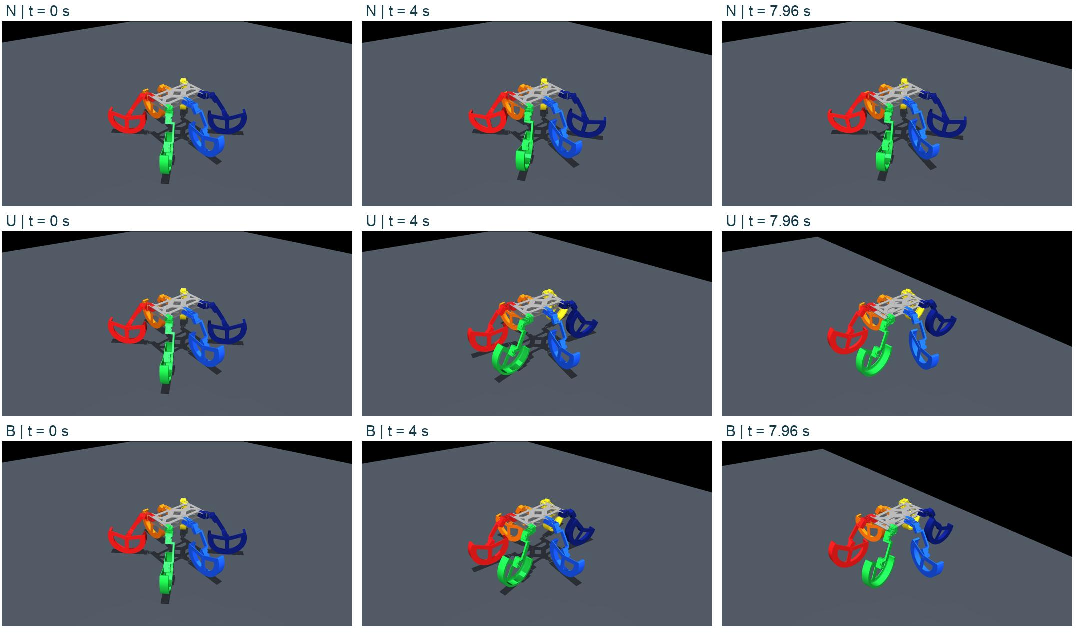
\includegraphics[width=.97\textwidth]{replay.pdf}
\caption{Actual simulation replays at the high command, phase zero, using decomposed tire contacts. Rows show N, U, and B; columns show measurement times 0, 4, and 7.96 s. The camera follows the robot; speed is measured from model state. The colors show model components, not contact force. All replays are checked against the corresponding raw record.}
\label{fig:replay}
\end{figure*}

\section{Discussion}
The central result concerns feasible use of a finite sector. A geometric arc limit alone does not constrain the rate of a subsequent rewind. Equations~\eqref{eq:budget}--\eqref{eq:project} connect usable stance rotation to the available swing time, while~\eqref{eq:residual} preserves the commanded travel allocation after saturation. The experiments measure the cost of imposing this constraint and distinguish it from disabling rolling altogether. The ablations also show why a full walking trajectory is not interchangeable with the residual trajectory.

The result has a precise scope. The fixed home and slew guard constrain the sector component, whereas the articulated IK target may vary faster. A future controller should jointly constrain the summed motor trajectory, account for measured tracking lag, and choose swing endpoints under actuator and support constraints. The present geometric role rule is inexpensive but does not optimize forces, stability margins, or energy. Constant-command tests characterize operating points; they are not a demonstration of autonomous navigation or robust transitions.

The contact decomposition resolves a specific collision inconsistency and enables future tests of concave edge interactions. It does not by itself establish an advantage in stair climbing. The physical archive in Fig.~\ref{fig:stairs} shows qualitative stair motion by an earlier prototype controller, with a visible cable and moving camera. There are no synchronized control logs, calibrated riser measurements, repeated trials, or electrical measurements linking that recording to B. Its role here is to document the mechanism's physical embodiment.

\begin{figure*}[t]
\centering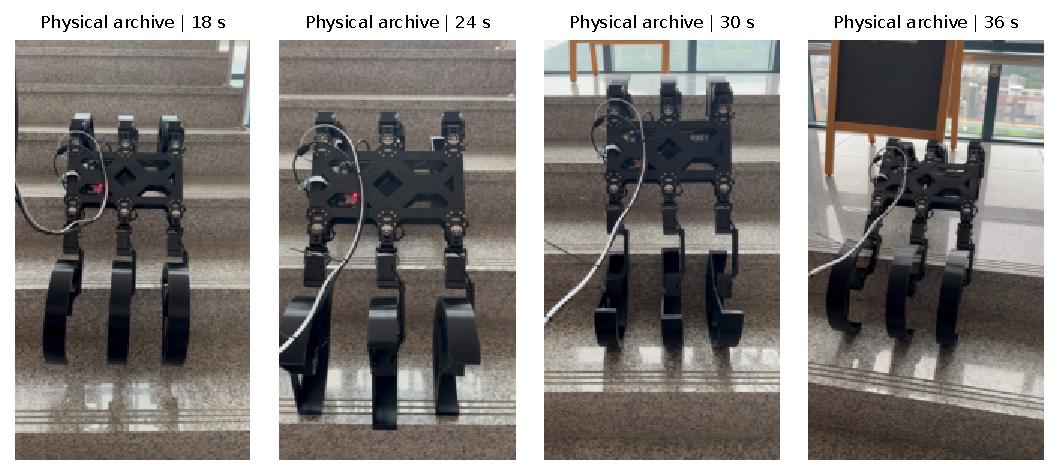
\includegraphics[width=.97\textwidth]{hardware_stairs.pdf}
\caption{Historical prototype stair sequence at source times 18, 24, 30, and 36 s. Original frame order, cable, and scene are retained. This qualitative recording is separate from the new simulation evaluation and does not quantify the proposed controller's stair performance.}
\label{fig:stairs}
\end{figure*}

The model retains rigid tire parts and nominal friction. Most link and motor collision geoms are disabled, and hinge hard stops are absent. Thus it does not establish whole-leg collision clearance, compliant contact behavior, thermal endurance, or hardware feasibility. The parameter stress cases and timestep comparisons probe numerical sensitivity within this model. Quantitative hardware experiments should compare B, U, and N under synchronized joint, pose, and current measurements before translating the simulated trade-offs into physical performance claims.

\section{Conclusion}
We presented a rewind-budgeted allocator for an articulated arc-leg hexapod. The method limits sector excursion by the available quintic swing time, enforces a discrete sector-rate bound, and assigns the remaining contact travel to articulation. A 268-trial simulation study with component restrictions and contact, command, and parameter checks quantifies its feasibility and transport trade-offs. The controller and concavity-preserving model provide a reproducible basis for subsequent hardware validation and concave-contact experiments.

\noindent\begin{minipage}{\columnwidth}
\section*{Acknowledgment of AI Assistance}
OpenAI Codex assisted with the Abstract, Sections I--VIII, source analysis, controller and evaluation code, and figure and video assembly. Numerical observations came from executed simulations or geometry calculations, and physical images from archival recordings. The authors must verify the final manuscript, references, code, and media before submission.
\end{minipage}
\par
\interlinepenalty=10000
\IEEEtriggeratref{10}\bibliographystyle{IEEEtran}\bibliography{references}
\end{document}
